\subsection{External interface requirements}
\subsubsection{User interfaces}
This section puts focus on the relation between the user and the mobile application. For better understanding the functionality of the application and the interaction with the user, beneath there are some mockups that represent a basic idea of what the mobile app will look like.

\begin{center}
\begin{minipage}[c]{.40\textwidth}
\centering
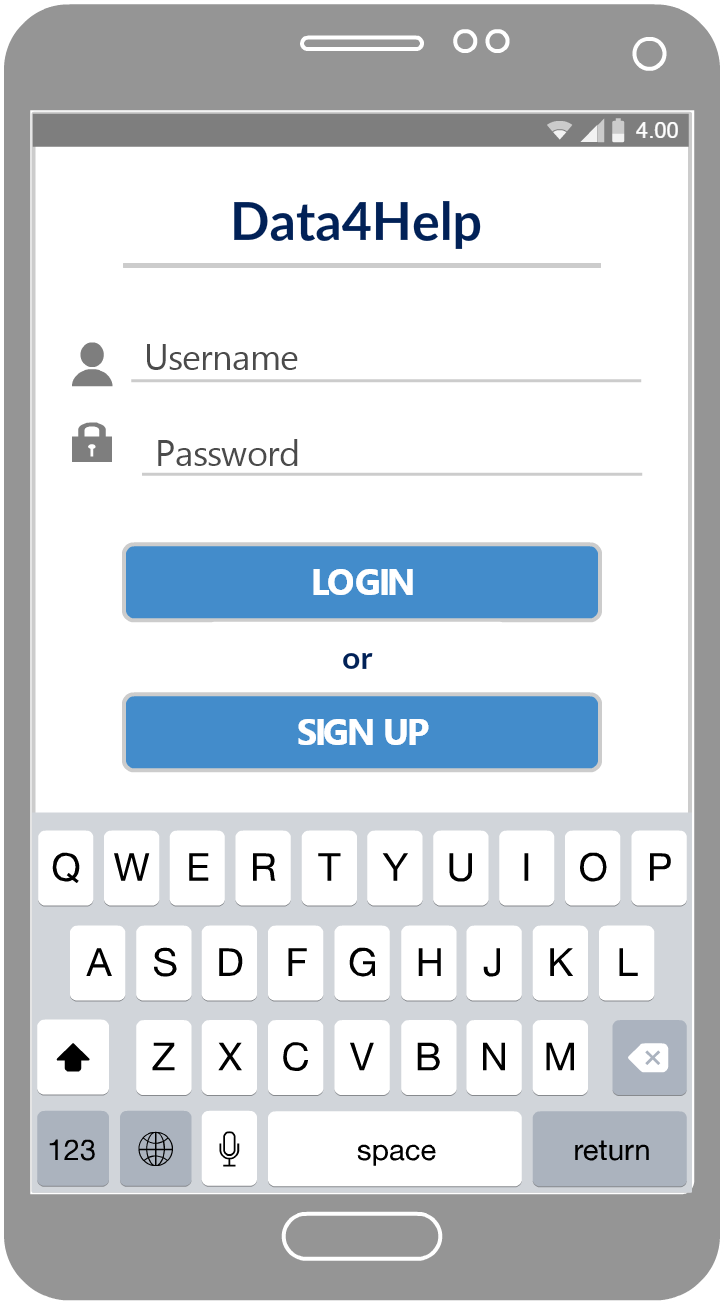
\includegraphics[width=1\textwidth]{Images/userInterface/Login}
\captionof{figure}{Mock up: Login.}
\end{minipage}%
\hspace{10mm}%
\begin{minipage}[c]{.40\textwidth}
\centering
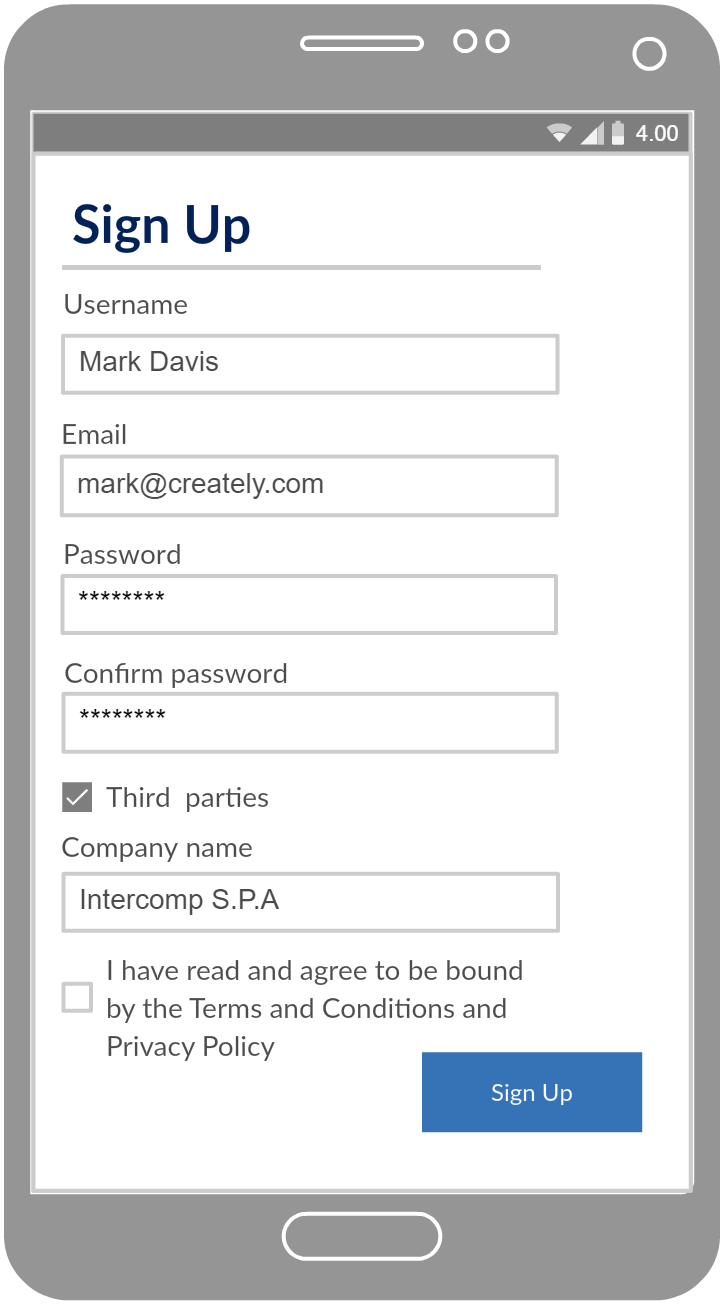
\includegraphics[width=1\textwidth]{Images/userInterface/SignUp}
\captionof{figure}{Mock up: Sign up.}
\end{minipage}
\end{center}
  
\begin{center}
\begin{minipage}[c]{.40\textwidth}
\centering
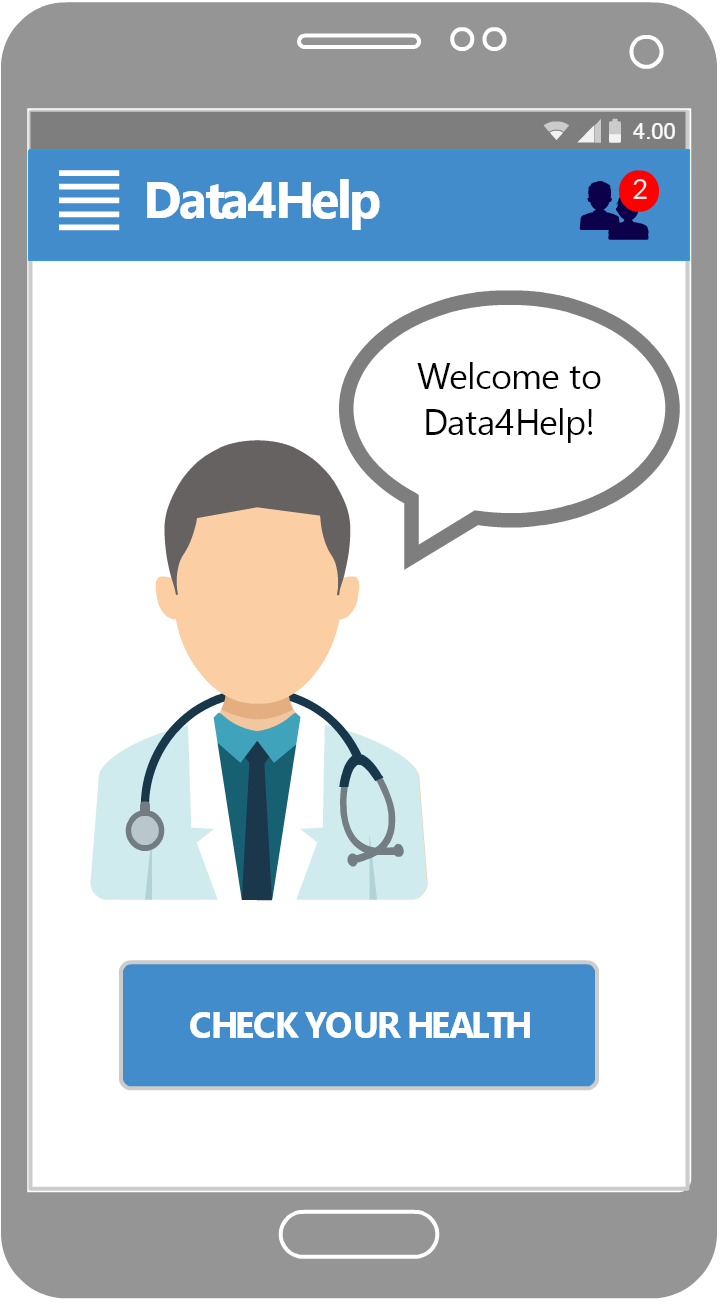
\includegraphics[width=1\textwidth]{Images/userInterface/Home}
\captionof{figure}{Mock up: Home.}
\end{minipage}%
\hspace{10mm}%
\begin{minipage}[c]{.40\textwidth}
\centering
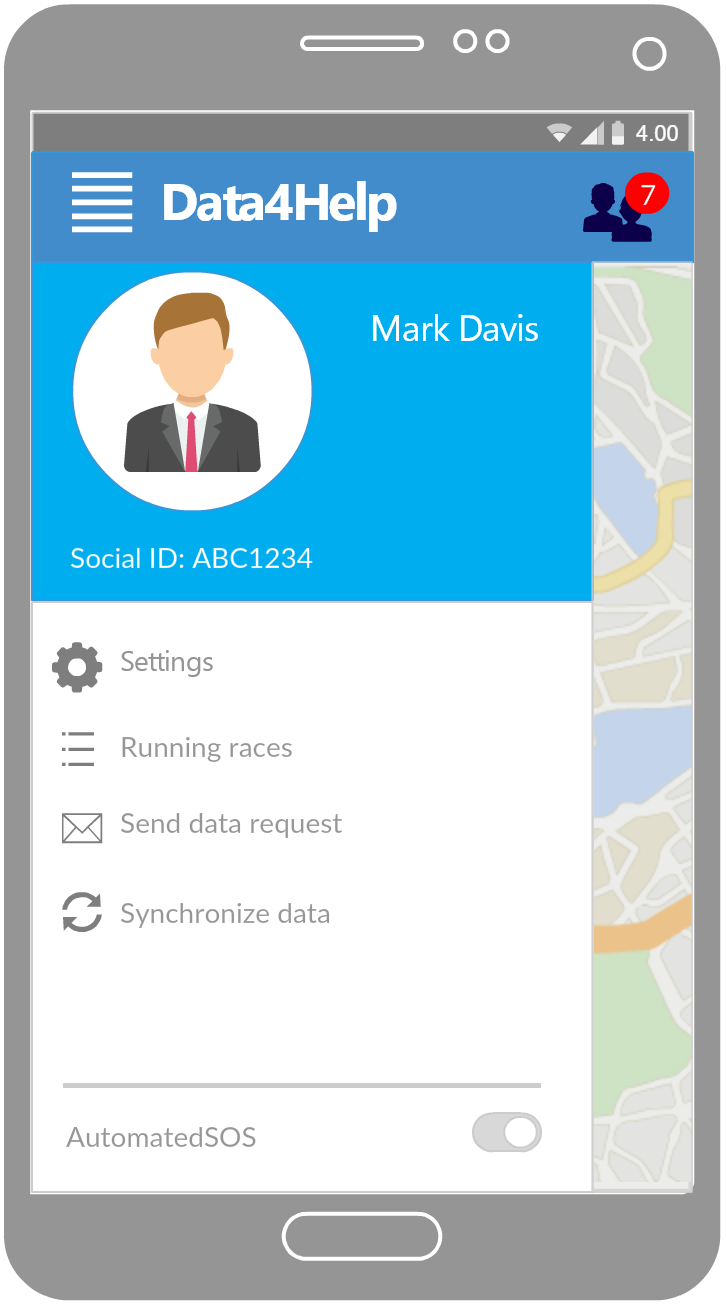
\includegraphics[width=1\textwidth]{Images/userInterface/MainMenu}
\captionof{figure}{Mock up: Main menu.}
\end{minipage}
\end{center}

\begin{center}
\begin{minipage}[c]{.40\textwidth}
\centering
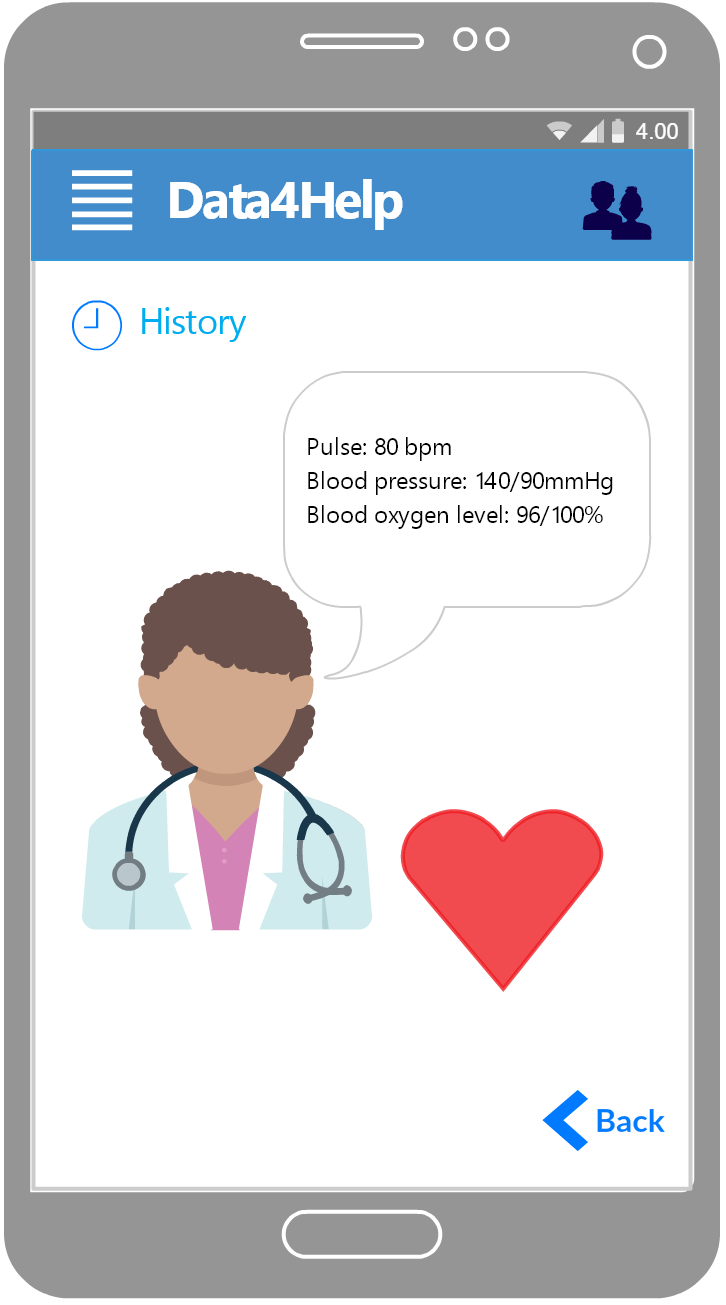
\includegraphics[width=1\textwidth]{Images/userInterface/HealthStatus}
\captionof{figure}{Mock up: Health status.}
\end{minipage}%
\hspace{10mm}%
\begin{minipage}[c]{.40\textwidth}
\centering
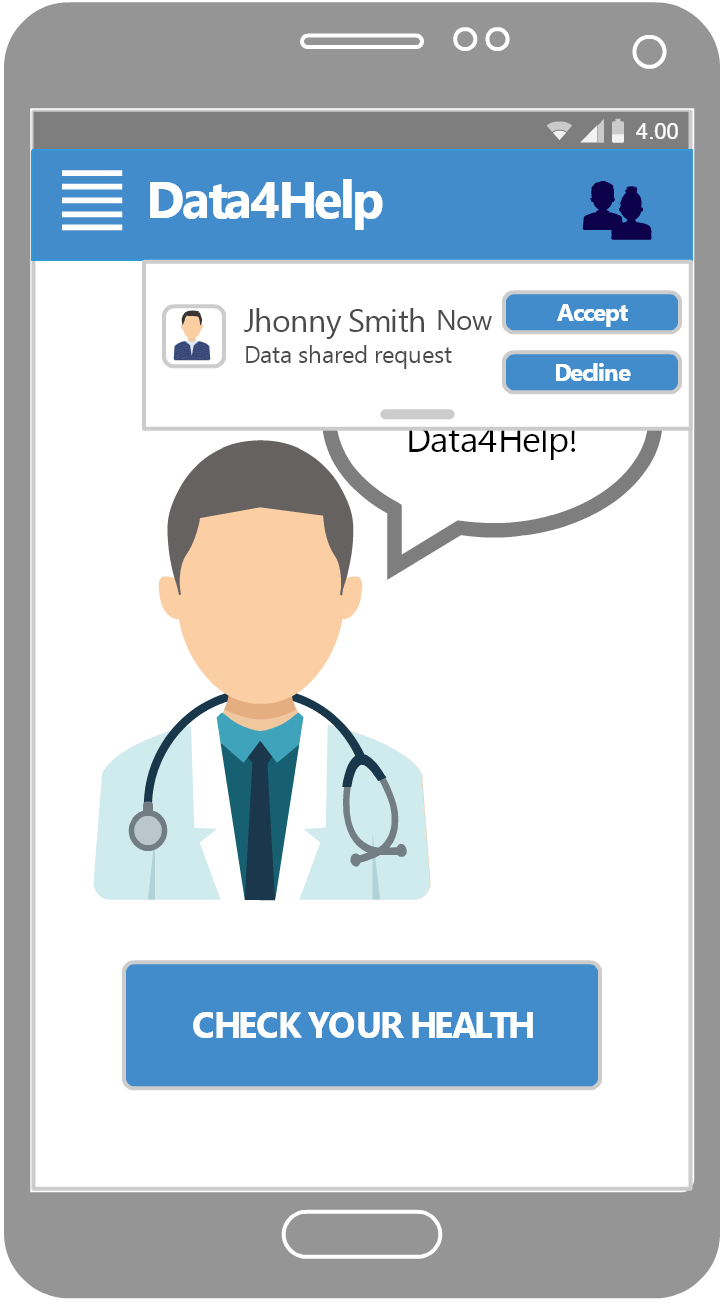
\includegraphics[width=1\textwidth]{Images/userInterface/ManageRequest}
\captionof{figure}{Mock up: Manage the request.}
\end{minipage}
\end{center}

\begin{center}
\begin{minipage}[c]{.40\textwidth}
\centering
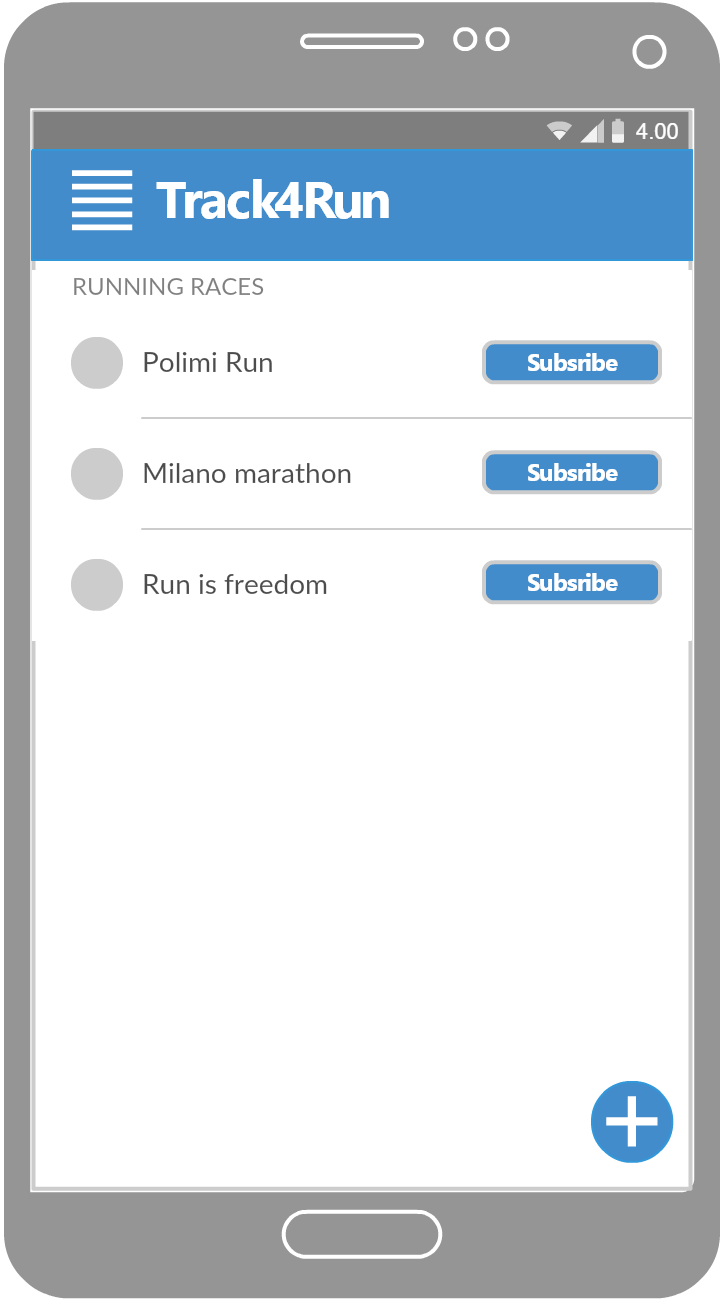
\includegraphics[width=1\textwidth]{Images/userInterface/RaceList}
\captionof{figure}{Mock up: List of available races.}
\end{minipage}%
\hspace{10mm}%
\begin{minipage}[c]{.40\textwidth}
\centering
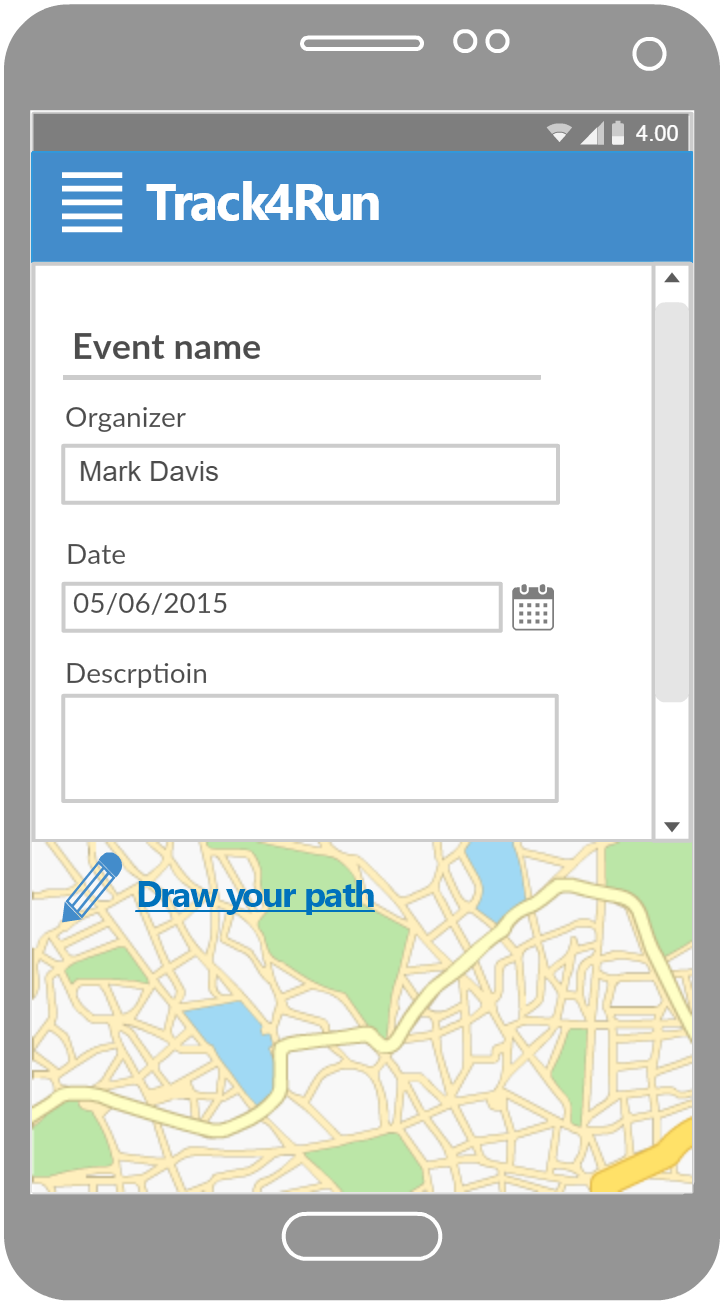
\includegraphics[width=1\textwidth]{Images/userInterface/AddEvent}
\captionof{figure}{Mock up: Add some events.}
\end{minipage}
\end{center}

\begin{center}
\begin{minipage}[c]{.40\textwidth}
\centering
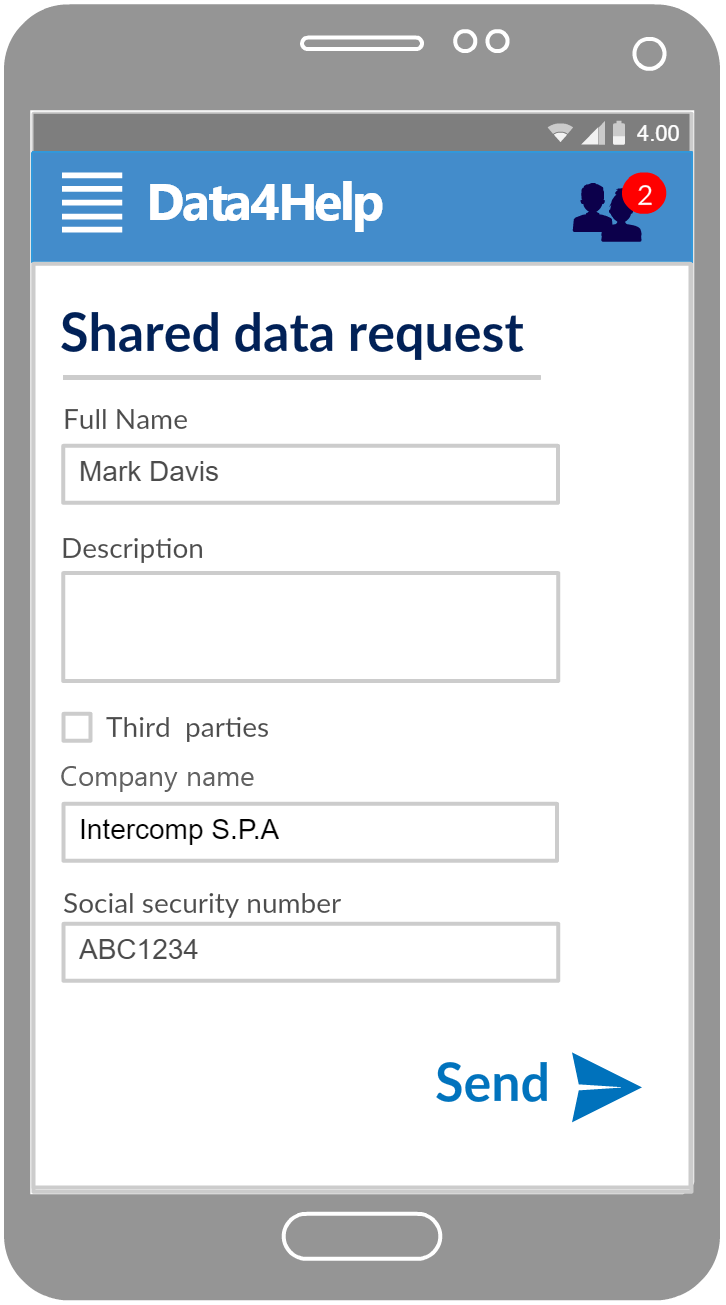
\includegraphics[width=1\textwidth]{Images/userInterface/SendRequest}
\captionof{figure}{Mock up: Shared data request form.}
\end{minipage}%
\hspace{10mm}%
\begin{minipage}[c]{.40\textwidth}
\centering
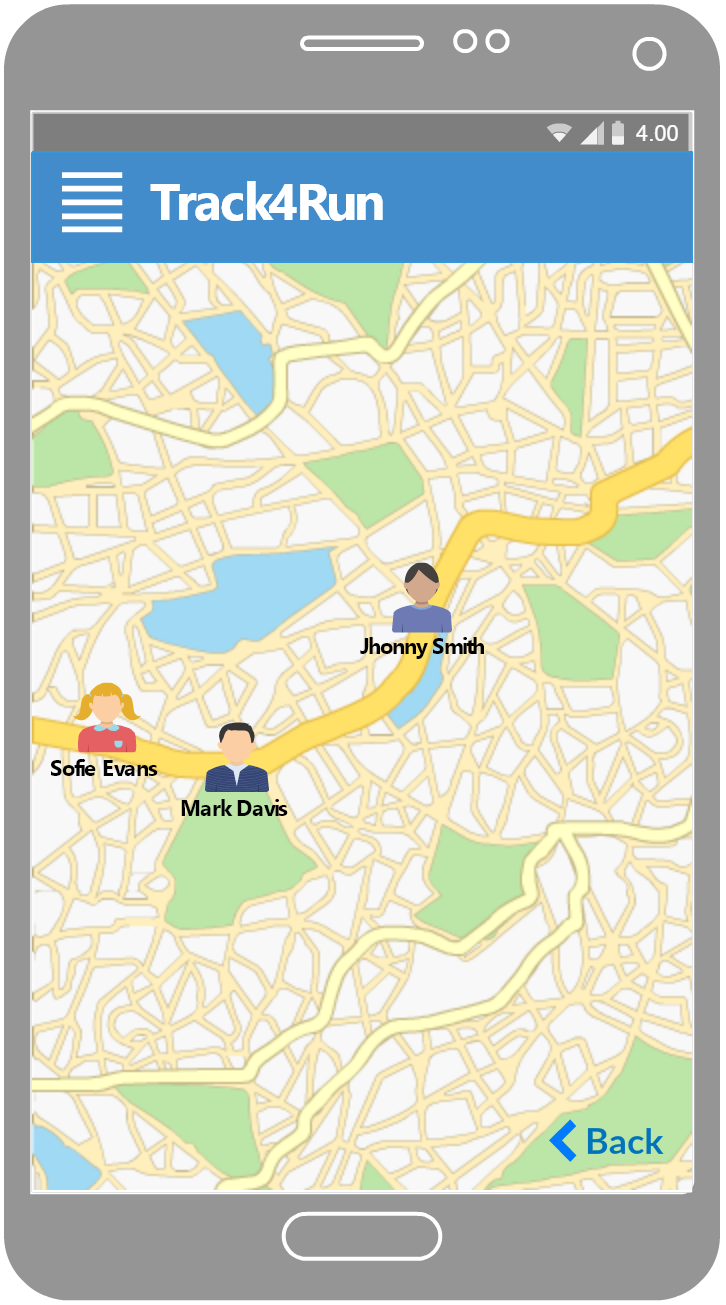
\includegraphics[width=1\textwidth]{Images/userInterface/Race}
\captionof{figure}{Mock up: Competition view.}
\end{minipage}
\end{center}
\subsubsection{Hardware interfaces}
The hardware part is mainly for heart rate, blood pressure and blood oxygen saturation levels data acquisition. It also plays a part in forwarding data to an Android phone by having an NFC tag. The software part, on the other hand, is responsible for data receiving and data processing. The software application running on an Android device aims at receiving, storing and utilizing the data. After data is written to the NFC tag, an Android phone will read the tag when it is close in range. Then the measurement process in the application will start and continuously obtain data from the NFC smartwatch or from the NFC tag inside the smartphone. Indeed this hardware structure can be implemented on a smartwatch / smartring or directly on the smartphone, but in this case the data acquisition will not be continues.
\begin{figure}[h!]
  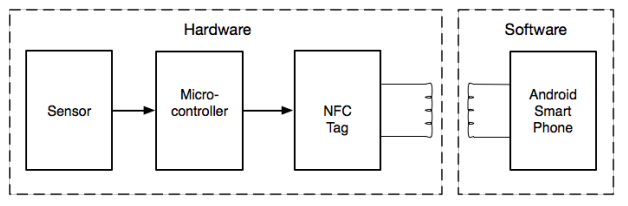
\includegraphics[width=\linewidth]{Images/hardware}
  \caption{The System Architecture.}
  \label{fig:The System Architecture}
\end{figure} 
The device must have also a GPS system for providing the position, a monitor for allowing, during the race, with the additional feature Track4Run, to see the athletes on the path, and finally the device must be able to call the 118 number.

\subsubsection{Software interfaces}
The application uses external service for reducing dependency on implementation specifics and makes code more reusable.
\begin{enumerate}
\item Race map\\
The application requires a usage of map for defining a path for the race and for seeing the position of the runner, during the competition. One options here is using Google Maps API which lets to customize maps with owner content and imagery for display on mobile devices. The Maps API features can modify using layers and styles, controls and events, and various services and libraries. This makes it perfect for being introduced in the Track4Run feature, since the users then can watch the competition directly on their smartphone by following the athletes on the path traced on the map. 
\item Call service\\
The smartphone's call service installed on the device is used by the application due to call the emergency number.
\item GPS Data service\\
The GPS Data as a Service API allows developers to store, handle, and manage GPS data in the system. GPS Data as a Service analyzes GPS data in real time so that application can use it to provide the position during the call to the emergency room operator and during the running race. It can also provide reports on analyzed data. 
\item Automated call\\
Automated call service allows, to AutomatedSOS, to call the emergency number and to speak with the operator.
Maybe the best option for recognizing the answer provide by the emergency room operator is the Google Cloud Speech API, that enables the AutomatedSOS feature to convert audio to text by applying neural network models in an easy to use API. The API recognizes over 80 languages and variants, to support your global user base. The API returns a list of two data.frame transcript and timings. The transcription frame contains the answer of the call, while in the timings frame there is a timetable with the word analyzed and the receiver's time. 
\item Text-to-speech\\
The Text-to-Speech API is ideal for any application that plays audio of human speech to users. It allows the application to convert arbitrary strings, words, and sentences into the sound of a person speaking the same things. For example in this case the API is used for reading, a formatted text message, during the call to the emergency number. The message provide all the information that usually required by the health staff. In addition, the language of the speaker can be chosen in the application preferences (english by default). One possible API for this interface can be Google test-to-speech.
\end{enumerate}
\subsubsection{Communication interfaces} 
The application project needs to several communication interface, indeed it continuously takes data information from the other devise, like smartwatch or sensor and, after a initially elaboration, it shares it with the core system. Moreover, with the feature AutomatedSOS, the App. needs to an specific interface for performing call. Summarize the Data4Help service has :
\begin{enumerate}
\item A communication interface for reading/writing data from the NFC tag. Fortunately the technology already has a specific protocol for this called NFC protocol.
\item A communication interface for sending and receiving data into the network, in order to interact with the core system. One possible solution is used the protocol HTTPs, that guarantees data security during the upload and download operations. 
\item A communication interface for performing calls. 
\item Some possible communication interfaces that allow to reach the goals of the application, discussed above in the software interface section.
\end{enumerate} 
